\section{What you are receiving}
You can open a recognizable, photo-inspired campus courtyard containing two parked quadrotors. The package contains the world, all project-specific geometry and materials, a ROS launch file, reusable terminal commands, verification tools, provenance records and this guide's exact LaTeX source. The software was actually built and loaded with the world paused. The screenshot below came from Gazebo's screenshot service, not an illustration generator.

\begin{figure}[htbp]\centering
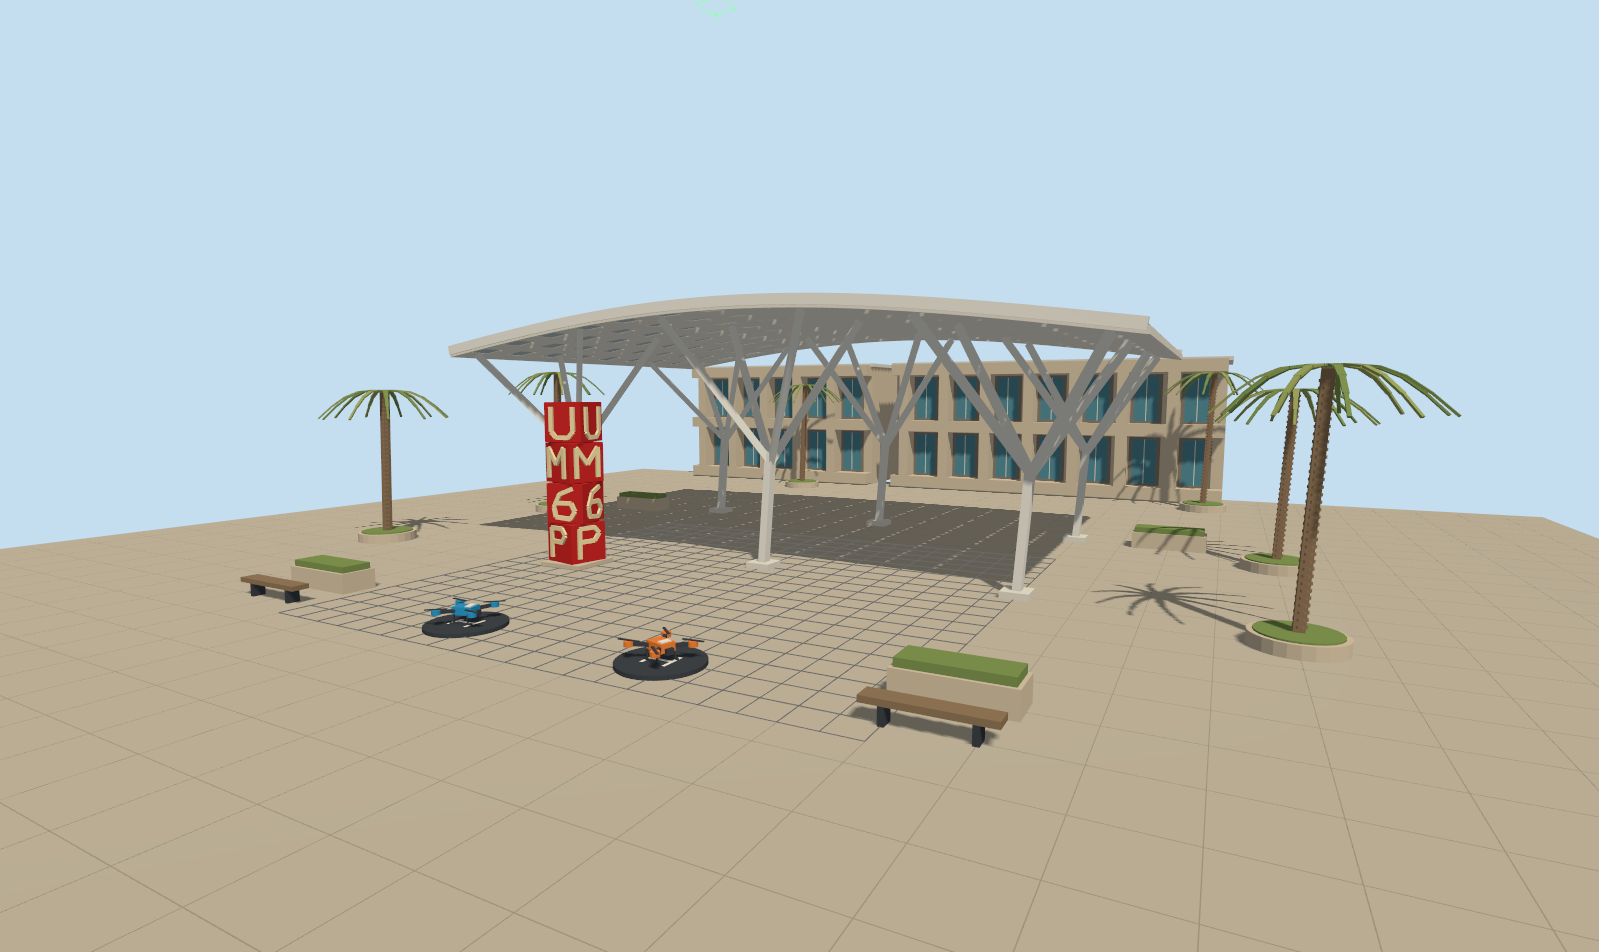
\includegraphics[width=\linewidth]{assets/campus-gazebo.png}
\caption{Actual Gazebo Harmonic rendering after the material and shutdown corrections. The blue and orange static quadrotors sit on separate pads. This view emphasizes the lattice and landmark.}\end{figure}

This is a recognizable architectural reconstruction, not a surveyed digital twin. Dimensions are assumptions. The four red blocks carry hand-modeled U, M, 6 and P shapes on two visible faces. No official UM6P logo asset is claimed. The original photographs were supplied by the researcher; their hashes are retained, but they are not redistributed because their source and redistribution rights were not supplied.

\subsection{Keep the scientific boundary clear}
The original campus inspection used Model 0-D v1.4. The current repository context is v1.6, titled \emph{Constraint Consensus-Based Dynamics for Decentralized Path Planning in UAV Swarms}. Scientific documents remain untouched. This decorative scene does not replace the mathematical workspace, obstacles, UAV radii or numerical benchmark.

The later Attempt 3 report supersedes the older two-attempt status: it reports numerical/TCC success and exact saved-plan safety certification, while the exact first-block Sun--Sun oracle failed. Thus the numerical campaign is not fully algorithm-certified. U3/U4 were resolved in the later research context. These are repository findings, not results produced by this environment task. No campaign trajectory is replayed here. Static visual separation does not certify Model 0-D safety.

This guide covers the parked environment only. The separately authorized kinematic demonstrations have their own guide and scenario folders; their existence does not change the paused campus launch.

\section{The software, in everyday terms}
\begin{description}
\item[ROS 2] A set of tools that lets separate programs exchange typed messages and services. Here it starts the environment and receives one informational test message. A running ROS program is called a node.
\item[Gazebo] A program for constructing and displaying virtual worlds. It can also compute physics, but this environment intentionally omits the Physics system and stays paused.
\item[ros\_gz] The official integration packages between ROS 2 and Gazebo. The bridge translates selected message types between their two communication systems.
\item[Workspace] A folder where related ROS packages are built and installed together. This delivered folder is the workspace root.
\item[Package] A named unit of ROS software or assets with a dependency manifest. Two packages define the parked campus; three more provide the demos.
\item[Launch file] A Python configuration that tells ROS which processes to start and which installed files to use. It is not a flight program.
\item[SDF world] An XML description of a world and its included models, lighting and systems. SDF means Simulation Description Format. This project does not need URDF.
\item[Mesh and material] A mesh is a collection of triangles defining a shape. A material defines its color and surface appearance. OBJ and MTL files store these locally.
\item[Build and install] Building prepares the packages. Installing copies their assets and configurations to the workspace's own install directory and creates the package index used at launch.
\end{description}

Loading a paused world creates the scene and communication endpoints. Rendering produces images using the graphics card. Neither requires time to advance in the physical simulation. Wall time still passes while you inspect a paused scene. This distinction is why the bridge check uses an informational message instead of requiring a continuously advancing clock or camera sensor stream.

\section{Chosen versions and prerequisites}
\begin{center}\begin{tabular}{p{.30\linewidth}p{.60\linewidth}}\toprule
Component & Observed in this execution session\\\midrule
OS and architecture & Ubuntu 24.04.5 Noble, x86\_64 / amd64\\
ROS distribution & ROS 2 Jazzy Jalisco, existing apt installation\\
Gazebo & Harmonic, Sim 8.15.0\\
Integration & ros\_gz 1.0.24 (full Debian revisions recorded)\\
Graphics & Intel Iris Xe ADL GT2, Mesa 25.2.8, OpenGL 4.6\\
Build tools & Python 3.12.3, GCC 13.3.0, ament\_cmake and colcon\\\bottomrule
\end{tabular}\end{center}

The official compatibility page recommends the Jazzy--Harmonic pairing on Ubuntu 24.04. Jazzy and Harmonic are supported through May 2029 according to the checked official release tables. They are not described here as the newest releases. Jazzy's official Gazebo vendor packages provide the matching libraries; a second Gazebo repository is unnecessary for this route.

The user's confirmed target is a Dell Latitude 5430, Intel i5-1245U, 16 GiB RAM and Intel Iris Xe graphics, using Ubuntu 24.04 Noble and Wayland with XWayland. The user supplied older package observations of Gazebo 8.11.0 and ros\_gz 1.0.22. Those observations are distinct from this session's measured 8.15.0 and 1.0.24. The task did not upgrade any installation. Older patch versions were not tested. Recheck the versions in your next local terminal session.

Docker and Podman were not available. The compatible native stack was already installed, so a native isolated workspace is the single maintained route. No container image, digest or dev-container test is claimed. Interactive VS Code execution is documented but was not tested through its UI. Approximately 125 GiB of disk space was available at inspection; the source assets are small, but optional TeX packages can require substantially more space than the campus itself.

\subsection{Command conventions}
All commands below are for Bash. Lines in a code box are commands unless explicitly labeled as output. Do not type a leading dollar prompt. Replace example paths with your own folder. Quote paths, especially when they contain spaces. Except where a different working directory is stated, run commands from the extracted \texttt{ros2\_gazebo\_um6p\_campus} root. Every provided wrapper locates its own root and sources ROS; it does not depend on a previous shell session or edits to your shell startup file.

\subsection{Enter and inspect the folder}
Prerequisite: the archive has been extracted. Working directory: any Bash terminal. Purpose: enter the delivered workspace and inspect the OS, disk and installed tools.
\begin{lstlisting}
cd "/your/path/ros2_gazebo_um6p_campus"
bash scripts/check_environment.sh
bash scripts/setup.sh --plan
\end{lstlisting}
The first line changes directory and normally prints nothing. The environment script prints OS, architecture, free space, tool paths and package versions. The setup plan makes no host changes. Observed setup output in this session was:
\begin{lstlisting}
All required packages already installed; no changes.
\end{lstlisting}
If \texttt{/opt/ros/jazzy/setup.bash} is absent, use the fresh Ubuntu setup subsection. If a required package is missing, the plan prints its name. Do not interpret a missing command in an unsourced shell as proof that ROS is not installed.

\subsection{Install only missing prerequisites on an existing ROS machine}
Prerequisites: Ubuntu 24.04 amd64, the official ROS apt repository already configured, internet access, and your decision to authorize the displayed package-manager transaction. Working directory: workspace root. Purpose: fill missing dependencies without upgrading already installed packages.
\begin{lstlisting}
bash scripts/setup.sh --install-missing
\end{lstlisting}
Expected result: either the no-change message, or apt's proposed installation followed by completion. The script uses sudo only in this explicit mode. It updates repository metadata and uses \texttt{--no-upgrade}. Read apt's proposed changes before accepting. This installation mode was not exercised here because no packages were missing. The underlying list is imported in the appendix.

\subsection{Fresh Ubuntu target: official repository setup}
This subsection is optional for a new, separately prepared Ubuntu 24.04 amd64 machine; skip it on the confirmed existing laptop installation. Provisioning a clean OS was not tested in this task. Working directory: any terminal for the first block. Prerequisites: administrator access, internet, and a normal Ubuntu installation with the appropriate Noble updates enabled. Purpose: enable Universe and obtain the official ROS apt configuration. These commands change host package sources and require an explicit operator decision.
\begin{lstlisting}
sudo apt-get update
sudo apt-get install curl software-properties-common
sudo add-apt-repository universe
\end{lstlisting}
The update refreshes the package index, installation supplies the two utilities, and the last command enables Ubuntu's Universe component. Expected result: successful package-manager output; none is claimed as observed here.

The official \href{https://github.com/ros-infrastructure/ros-apt-source/releases/tag/1.3.0}{ros-apt-source release 1.3.0} was checked through GitHub. Working directory: workspace root. Prerequisites: the utilities above, internet and approval for repository configuration. Purpose: download the exact Noble package, verify its published SHA-256, install the repository configuration and then the campus prerequisites.
\begin{lstlisting}
mkdir -p .runtime/setup
curl --fail --location \
  "https://github.com/ros-infrastructure/ros-apt-source/releases/download/1.3.0/ros2-apt-source_1.3.0.noble_all.deb" \
  --output .runtime/setup/ros2-apt-source.deb
sha256sum .runtime/setup/ros2-apt-source.deb
\end{lstlisting}
The first command creates a local download folder; the second retrieves the versioned package; the third prints its checksum. Expected SHA-256 from the official release metadata:
\begin{lstlisting}
f31d84adf5054c7d60ded0e82c0f776a77ea33af53d08f40b9ad7c94cca55296
\end{lstlisting}
Proceed only if the printed hash agrees. Same working directory and prerequisites; purpose: explicitly install the repository configuration and missing dependencies.
\begin{lstlisting}
sudo dpkg -i .runtime/setup/ros2-apt-source.deb
bash scripts/setup.sh --install-missing
\end{lstlisting}
Expected result: repository configuration succeeds, then apt proposes any needed runtime packages. No fresh-OS setup, repository modification or host update was executed here. Exact apt dependency availability can change even though this repository-setup package is pinned. If Noble update suites or dependencies conflict, inspect the official ROS installation instructions rather than applying an unreviewed full system upgrade.

\section{How the directory is organized}
\begin{center}\small\begin{longtable}{p{.35\linewidth}p{.56\linewidth}}\toprule
Location & Purpose\\\midrule\endhead
\texttt{README.md} & Short entry point and exact commands.\\
\path{campus_environment/src/um6p_campus_description/} & Package manifests, local models, meshes/materials and SDF world.\\
\path{campus_environment/src/um6p_campus_bringup/} & Installed launch, bridge, server and saved camera configuration.\\
\texttt{scripts/} & Shared entry points; the campus generator is in campus\_environment/scripts/.\\
\texttt{campus\_environment/tests/} & Installed asset validation and bounded runtime checks.\\
\texttt{.vscode/} & Task definitions that call the same shell scripts.\\
\texttt{docs/} & Assumptions, scene manifest, local target and reproducibility notes.\\
\texttt{references/} & Repository identities, photo provenance, dependency lists and official sources.\\
\texttt{evidence/} & Actual logs, JSON results, screenshots and verification record.\\
\texttt{tutorial/} & Two named PDFs; exact sources and figures under source/.\\
\texttt{decisions/} & Environment-scope record only; not a mathematical decision.\\
\texttt{checkpoints/} & Durable status and next actions for recovery.\\
\texttt{build/, install/} and\newline\texttt{log/, .runtime/} & Generated local work, ignored for publication.\\\bottomrule
\end{longtable}\end{center}
The folder can later be placed as one new top-level directory in the repository. Nothing in the scientific baseline needs moving. The repository branch was inspected through a pinned connector snapshot at commit \texttt{e3a8af05cbb40793f6b48f26ffe042dc51f0ddca}. A terminal Git clone failed private-repository authentication. The delivery is therefore a dedicated environment directory, not a claimed complete Git checkout.

\section{Build, launch, inspect and stop}
\subsection{Build installed packages}
Working directory: workspace root. Prerequisites: the dependency plan passes. Purpose: build and install all five project packages locally.
\begin{lstlisting}
bash scripts/build.sh
\end{lstlisting}
Expected result: colcon reports five packages finished. The current reorganized build completed all five packages successfully. Repeating this command is safe: colcon updates only generated workspace outputs. The script does not use a symlink install; copied installed assets are the runtime source. The package CMake files install their required directories.

\subsection{First bounded verification}
Working directory: workspace root. Prerequisite: build completed and no other campus test is running in ROS domain 84. Purpose: validate installed resources, then load and close the paused world twice.
\begin{lstlisting}
bash scripts/verify.sh headless
\end{lstlisting}
Expected result: asset JSON with \texttt{status: PASS}, then runtime JSON with \texttt{status: PASS}. Evidence is saved under \texttt{evidence/local-headless/}. This command has a 120-second overall timeout and bounded sub-operations. It does not open a graphics window. Failure produces a nonzero exit and a result or console error; inspect the saved logs before retrying.

\subsection{Open the default camera view}
Working directory: workspace root. Prerequisite: build passed and a working graphical session is available. Purpose: open the paused courtyard.
\begin{lstlisting}
bash scripts/launch_environment.sh gui
\end{lstlisting}
Expected result: Gazebo displays the underside of the pergola, four letter blocks, buildings and both UAVs. The terminal stays occupied while it owns Gazebo and the bridge. There are no play, step, spawn or transform controls in the supplied GUI. Use camera navigation to inspect the scene only. Do not send world-control commands from another client. Gazebo's built-in generic services still exist; the configuration is a workflow boundary, not an adversarial security barrier.

To close the scene, return to the launching terminal and press \textbf{Ctrl+C once}. Wait for messages that Gazebo and the bridge finished cleanly. This sends the interrupt to the launch owner, which manages its children. Repeated interrupts or killing the entire process group while ROS also forwards interrupts caused an initial wrapper error during development; the test helper was corrected to signal the owner once.

\subsection{Other saved view and automatic visual check}
Working directory: workspace root. Prerequisite: the preceding launch has shut down. Purpose of the first command: use the overview camera. Purpose of the second: automatically test two GUI launches and save an actual screenshot. Run them separately, stopping the first with Ctrl+C before the second.
\begin{lstlisting}
bash scripts/launch_environment.sh gui overview
bash scripts/verify.sh gui
\end{lstlisting}
The overview should reveal more of the full canopy footprint and landscaping. Its configuration is included; the final corrected default camera is the one formally verified and pictured in this guide. Before capturing evidence, the verifier resets the GUI camera to the pose stored in the installed configuration using a camera-only service. It also requires an actual saved PNG. The GUI verification saves under \texttt{evidence/local-gui/} and exits automatically. A screenshot-service reply is not enough to establish visual quality: open the PNG and inspect it.

\subsection{Direct installed ROS use}
For readers who want to understand the wrapper: working directory can be any directory after adjusting the workspace path below. Prerequisites: a successful build and no conflicting launch. Purpose: load the official and project package indexes, then invoke the same installed launch file.
\begin{lstlisting}
source /opt/ros/jazzy/setup.bash
source "/your/path/ros2_gazebo_um6p_campus/install/setup.bash"
export ROS_DOMAIN_ID=84
export ROS_AUTOMATIC_DISCOVERY_RANGE=LOCALHOST
export GZ_PARTITION=ccbo_campus
ros2 launch um6p_campus_bringup campus.launch.py gui:=true
\end{lstlisting}
The source commands normally print nothing. They make installed package names resolvable. The environment variables restrict ordinary ROS discovery and select a Gazebo partition. The final line opens the same world. Prefer the wrapper for normal use because it also places logs under the workspace. Stop with Ctrl+C. No command in this guide uses Gazebo's run-on-start flag.

\section{How the scene was constructed}
\subsection{Assumptions and dimensions}
The paved courtyard is 64 by 60 metres, centered at $(0,5)$; its visible top is $z=0$. The main canopy covers $x\in[-14,14]$ and $y\in[0,18]$. Its gentle transverse curve is
\[
 z(x)=8.6+1.35\cos(\pi x/28)\quad\text{metres}.
\]
This gives 8.6 m at the edges and 9.95 m at the crest. One-metre roof segments approximate the curve. Repeated beams at roughly two-metre spacing form the visible structural lattice. There are six branching support assemblies at $x=-10,0,10$ and $y=3,15$. Trunks rise from broad feet, then split into four diagonal arms.

Following the researcher's layout feedback, both buildings are translated 12 m farther along $+Y$, leaving a 13.8 m clear horizontal gap between the pergola edge and the front facade bands. The existing palms, planters, benches, paving and pergola geometry remain unchanged. Two stone-colored rear building volumes are about 16 and 22 m wide, 8 m deep and 9 m high. Their facade columns and horizontal bands stand in front of dark window recesses and blue glass surfaces. This gives real geometric depth without detailed interiors. Six simplified palms, raised planting beds and benches provide restrained landscaping. A directional warm sun supplies shadows. These dimensions are artistic assumptions, not a survey or a load-bearing structural design.

The landmark is at $(-7,0,0)$, on a small plinth. Four 1.6 m blocks stack vertically with visible narrow gaps. The generator builds them bottom-up as P, 6, M, U; reading the finished tower top-down yields U, M, 6, P. The blocks alternate $+12$ and $-12$ degrees around their vertical axes: U and 6 share one orientation, M and P the other. Each block and its letters rotate together. This follows the additional UM6P photograph supplied in the feedback; angles are artistic estimates. Each letter consists of local polygonal strokes on the front ($-Y$) and right ($+X$) faces. This approximates the supplied photograph without introducing an invented official logo file.

\subsection{Coordinates, names and UAV poses}
World coordinates are right handed: $+X$ points across the courtyard to the right in the design, $+Y$ toward the rear buildings, and $+Z$ upward. Units are metres and radians. There is no GPS datum or surveyed north. SDF poses are written in the order $x,y,z,\mathrm{roll},\mathrm{pitch},\mathrm{yaw}$.

\begin{center}\begin{tabular}{lll}\toprule
Model & Pose & Color\\\midrule
\texttt{uav\_1} & $(-3.6,-8.2,0.12,0,0,0.3)$ & Blue\\
\texttt{uav\_2} & $(3.6,-8.2,0.12,0,0,-0.3)$ & Orange\\\bottomrule
\end{tabular}\end{center}
Their origins are 7.2 m apart. The pads and UAVs occupy the open forecourt at $y=-8.2$, leaving room for future staging. An unmarked 18 by 18 m area, $x\in[-9,9]$ and $y\in[-22,-4]$, is kept clear of other above-ground scene objects. This 324 square metre reserve does not assert a flight capacity for 3, 5, 10, 20 or 100 UAVs. Future counts, body dimensions, pad spacing, trajectories and safety requirements must be separately reviewed; no additional vehicle or formation generator is active. The current world still contains exactly two UAVs. Each sits above a 0.12 m display pad. Landing skids start at local $z=0.005$, approximately 5 mm above the pad top; static geometry preserves this visual clearance without contact solving. Body boxes, four arms, motor cylinders and rigid propeller bars make the vehicles recognizable. The local body center is above the model origin; the listed model pose is not a calibrated center of mass.

The UAV meshes span roughly 1.8 m across including propellers. They are separated from one another, landmark and columns, but no certified safety claim follows. Their small body collision box is a placeholder only. Decorative architecture is visual geometry, not a validated collision environment. No mass, inertia, aerodynamic model or flight controller is validated.

\subsection{Generator and resources}
The full generator is imported in the appendix. Its \texttt{Mesh} helper writes triangles and surface normals for boxes, oriented beams and cylinders. The \texttt{Model} helper groups shapes by material, writes local OBJ/MTL files and builds static SDF models. Grouping keeps the scene to 25 meshes and 25,540 triangles rather than thousands of independent entities. The final world includes seven top-level models; only two are UAVs.

Working directory: workspace root. Prerequisite: Python 3 standard library; stop the scene before changing assets. Purpose: regenerate the first-party asset set from its maintained recipe, then reinstall it.
\begin{lstlisting}
python3 campus_environment/scripts/generate_assets.py
bash scripts/build.sh
bash scripts/verify.sh assets
\end{lstlisting}
Expected result: the generator reports seven static models; build installs them; validation reports PASS. The meshes need no texture images, fonts, Fuel cache or attachment files at runtime. OBJ references local MTL files, while SDF specifies the same colors. A deterministic regeneration hash check is included in the verification record. Changing scene dimensions requires rerunning the relevant asset and visual checks; it does not authorize changing the scientific model.

\section{ROS/Gazebo integration and test results}
The installed launch uses ament's package index to find resources. It runs Gazebo and a single node named \texttt{campus\_evidence\_bridge}. The bridge is one-way, Gazebo to ROS, on \texttt{/campus/evidence}, translating \texttt{gz.msgs.StringMsg} to \texttt{std\_msgs/msg/String}. This informational topic has no connection to UAV movement.

The runtime verifier requests \texttt{/world/um6p\_campus/scene/info} and checks the seven model names and UAV poses, including yaw quaternions. This is verified service exchange, not just endpoint discovery. It subscribes to world statistics and requires every sampled message to report paused, zero iterations, zero simulation time and no stepping. It also publishes a unique informational string through Gazebo transport and checks that the ROS subscriber receives that exact string. The ROS graph must contain only the bridge and the temporary verifier.

The launch omits Physics, Sensors and UserCommands systems. The only requested server system is SceneBroadcaster. Gazebo may print a default physics-profile name while initializing world metadata; that message does not mean the Physics system was loaded or physics advanced. The zero-iteration evidence and explicit system configuration are the relevant observations.

\begin{center}\begin{longtable}{p{.53\linewidth}p{.35\linewidth}}\toprule
Check & Outcome and evidence\\\midrule\endhead
Two packages build and install & PASS; build log.\\
World and seven model SDF files & PASS; installed asset validator.\\
25 local meshes and resource resolution & PASS; asset check and corrected GUI logs.\\
Exactly two UAVs and specified poses & PASS; scene service responses.\\
Informational Gazebo-to-ROS message & PASS; exact received strings recorded.\\
Paused, zero time/iterations, no stepping & PASS in all final sampled statuses.\\
Headless shutdown and relaunch & PASS; two launches.\\
Corrected default GUI rendering & PASS; actual PNG visually inspected.\\
Corrected GUI shutdown and relaunch & PASS; two clean child exits.\\
Fresh source rebuild in path with spaces & PASS; same installed dependencies, new build/install.\\
Fresh operating-system provisioning & NOT VERIFIED; no new OS installed.\\
Docker/dev-container & NOT VERIFIED; runtime absent, route not used.\\
Older user-reported package versions & NOT VERIFIED.\\
VS Code task UI & NOT VERIFIED; shared command workflow supplied.\\
Software-only/EGL rendering & NOT VERIFIED; hardware GUI rendering available.\\
Physics, sensors, dynamics, flight & OUT OF SCOPE; not executed.\\\bottomrule
\end{longtable}\end{center}

Initial failures and corrected attempts remain documented. The initial GUI material warnings and duplicate-interrupt child exit do not count as clean-shutdown success, even though the early test wrapper returned an overall PASS. The revised verifier checks child logs as well as its parent return code. Ordinary Qt dialog binding warnings remain; the final logs show no missing required assets, Gazebo error or failed child process.

\subsection{Portability check}
Working directory: workspace root. Prerequisites: installed dependencies and a nonexistent destination outside this folder. Purpose: reproduce the maintained source in a fresh location, including paths with spaces.
\begin{lstlisting}
bash scripts/reproduce_clean.sh "/new/path/campus clean copy"
\end{lstlisting}
Expected result: new build/install directories, successful asset validation, two paused campus launches and both separately authorized kinematic demo checks. This combined reproduction command advances demo time; it never advances the parked campus world. Existing destinations are rejected to preserve edits. The current check uses a new directory named \texttt{campus organized clean reproduction}, including spaces. It is a clean source rebuild on the same installed OS, not proof of clean-OS package provisioning or old-version compatibility.

\section{Visual Studio Code workflow}
Open VS Code and choose File $>$ Open Folder, selecting the delivered root. Open Terminal $>$ New Terminal. Use the same setup, build, verification and launch commands shown above. The integrated terminal uses the same installed ROS environment because the scripts source it explicitly.

Alternatively, use Terminal $>$ Run Task and select \texttt{Check prerequisites}, \texttt{Build}, \texttt{Verify campus headless}, or \texttt{Campus: launch paused}. The included tasks use process arguments, so workspace paths containing spaces are preserved. The launch terminal remains active. Stop it with Ctrl+C once, then wait for the child exit messages. No dev-container extension is required. This task configuration was inspected; no interactive VS Code UI run is claimed.

\section{Troubleshooting and safe cleanup}
\begin{description}
\item[ROS or Gazebo command not found.] Use the supplied scripts, which source the Jazzy installation. If the setup file truly does not exist, use the optional installation route. Do not install a second incompatible distribution simply because a fresh shell is unsourced.
\item[SDF include cannot be found.] Gazebo uses \texttt{GZ\_SIM\_RESOURCE\_PATH}; the standalone \texttt{gz sdf} checker additionally needs \texttt{SDF\_PATH}. The asset test sets it. Launch from the installed package after building, not by guessing a temporary source path.
\item[Blank window or display unavailable.] Check that the command runs inside your graphical desktop session. The execution sandbox initially could not access display :0; authorized host-side rendering worked without changing security settings. Do not disable access controls or change drivers as a first response.
\item[Transport getifaddrs error.] The sandbox denied network-interface discovery. The actual tests required permitted local transport access outside it. This is different from a missing ROS package. Do not disable host security settings to guess at a solution.
\item[No bridge message.] Do not unpause. Ensure the same partition and domain are used and run one verifier at a time. The verifier publishes its own text independently of physics. A listed topic is not proof of message delivery.
\item[Scene appears unchanged after edits.] Rebuild; runtime uses copied installed assets. Close old launch processes before opening the rebuilt scene.
\item[Material warnings.] The initial meshes lacked MTL references. The delivered generator writes both OBJ and matching MTL files. Regenerate and rebuild if either is missing; do not download unrelated materials.
\item[Version conflict.] Compare local versions with the manifests. Exact apt revisions may no longer be available. Preserve the error and seek a compatible reviewed installation instead of forcing a downgrade or mixing repositories.
\item[GUI wrapper error during shutdown.] Press Ctrl+C once in the owner terminal. The final verifier signals its owner once and checks child logs. Do not use a broad command that kills every Gazebo or Python process on the computer.
\end{description}

Working directory: workspace root. Prerequisite: all task-owned launch/test processes have stopped. Purpose: remove only generated workspace products so you can rebuild, retaining source, documentation and evidence.
\begin{lstlisting}
rm -rf -- build install log .runtime
bash scripts/build.sh
\end{lstlisting}
The deletion is intentionally relative to this workspace; confirm your current folder before using it. Expected result: generated outputs disappear and then build creates new ones. Do not delete your system ROS installation, scientific repository directories or archived evidence. This cleanup was documented, not run against the final working delivery.

\section{Provenance, versions and recovery}
The source folder records the starting branch commit, Git blob identities, attachment hashes, observed direct package pins, the complete installed package list and file checksums. No credentials or private authentication material are required by the runtime. Original source snapshots were kept outside the publication folder; the manifest links back to their exact repository commit.

A package list is not a permanent reproducibility lock. Apt repositories, TeX packages and website documentation remain mutable. Exact retained binary packages, repository metadata and an OS image would be needed for stronger long-term binary recovery. No container digest is applicable because no container is used. Installation downloads are distinct from runtime: every project-specific runtime asset is already included.

Working directory: extracted workspace root. Prerequisite: retain the delivery's checksum manifest. Purpose: confirm that the delivered files match the recorded bytes.
\begin{lstlisting}
sha256sum --check SHA256SUMS
\end{lstlisting}
Expected result: OK for every listed file. This identifies the delivered state, not an external signature or a certification of dynamics. The manifest excludes itself and disposable build/cache files. Rebuilds and new local verification folders do not invalidate maintained source hashes; intentional source changes do.

If work must pause, read \texttt{checkpoints/STATE.md} first on resumption. Confirm files and dependencies still exist, preserve intervening user edits, and continue from the exact saved next action. Do not assume a cache or process survives. No automatic credit-reset continuation is promised.

\section{Recompile this exact tutorial}
This PDF is compiled from the delivered LaTeX files. \texttt{listings.tex} imports complete first-party scripts and configurations from the actual delivered paths. The generator source replaces enormous repetitive mesh-coordinate listings; all generated geometry is still present as files and hashed.

Working directory: workspace root. Prerequisites: optional document compilation tools. Purpose: install a conventional Ubuntu LaTeX/PDF toolchain if you choose to do so. This optional host installation was not performed here.
\begin{lstlisting}
sudo apt-get install texlive-latex-recommended \
  texlive-latex-extra texlive-fonts-recommended \
  latexmk poppler-utils python3-pil
\end{lstlisting}
Expected result: a proposed apt transaction, then the tools installed after operator acceptance. Review disk requirements. The task used an available Tectonic executable and a copied cache inside task-owned storage rather than modifying the system TeX installation.

Working directory: workspace root. Prerequisite: latexmk or Tectonic available on PATH. Purpose: regenerate the appendix include list and compile the PDF.
\begin{lstlisting}
bash scripts/build_tutorial.sh
\end{lstlisting}
Expected result: \path{tutorial/01_UM6P_Campus_Environment_Setup_and_Coding.pdf} and PDF metadata. Compilation may download TeX support files if using Tectonic without a populated cache; these are documentation-time dependencies only. No scene runtime assets are downloaded.

Working directory: workspace root. Prerequisite: compiled PDF and Poppler. Purpose: render every page for visual inspection.
\begin{lstlisting}
mkdir -p tutorial/qa
pdftoppm -r 110 -png tutorial/01_UM6P_Campus_Environment_Setup_and_Coding.pdf tutorial/qa/page
\end{lstlisting}
Expected result: one PNG per PDF page. Open every page, check that code wraps within margins, headings and page numbers are readable, and figures and links are present. The final delivery includes a separate PDF QA record. Do not infer layout quality solely from successful compilation.

\section{What remains before future flight work}
This delivery prepares a paused scene. Future flight experiments require separate authorization and a reviewed design for vehicle dynamics, controllers, state estimation, coordinate alignment, collision geometry, timing, sensors, bridge interfaces and scientific protocol. The parked UAVs must be replaced or extended with validated vehicles. No previous numerical trajectory should be replayed simply because Gazebo now opens.

The researcher authorized publication of the reorganized delivery on 20 September 2026. The final checkpoint, verification record and separate publication receipt identify the handoff state. Scientific repository files outside this delivery remain unchanged.

\section*{Official references}
\addcontentsline{toc}{section}{Official references}
\begin{enumerate}
\item \href{https://gazebosim.org/docs/harmonic/ros_installation/}{Gazebo: Installing Gazebo with ROS}. Pairing and vendor-package route, rechecked 20 September 2026.
\item \href{https://www.ros.org/reps/rep-2000.html}{ROS REP 2000}. Supported platforms and Jazzy lifecycle.
\item \href{https://gazebosim.org/docs/harmonic/releases/}{Gazebo release table}. Harmonic lifecycle.
\item \href{https://docs.ros.org/en/jazzy/Installation/Ubuntu-Install-Debs.html}{ROS Jazzy Ubuntu apt installation}. Web page returned a bot challenge; its official \href{https://github.com/ros2/ros2_documentation/tree/jazzy/source/Installation}{GitHub documentation source} was inspected.
\item \href{https://docs.ros.org/en/jazzy/p/ros_gz_bridge/}{ros\_gz\_bridge documentation} and \href{https://github.com/gazebosim/ros_gz/tree/jazzy}{official source}. Installed headers, launch files and message bindings were also inspected.
\item \href{https://gazebosim.org/docs/harmonic/sdf_worlds/}{Gazebo SDF worlds}. Installed command help and SDF validators provided execution-time checks.
\end{enumerate}

\section{Organization and current verification}
The campus packages live in \path{campus_environment/src/}. The two demo packages live below \path{demo/}; their common code lives below \path{common/}. The root build script installs all five packages. This guide's source is in \path{tutorial/source/campus_environment/}; the other guide explains motion. User videos belong to their respective demo media folders. Generated build products are excluded from the source archive.

Current verification is recorded in \path{evidence/VERIFICATION_CURRENT.md}. Earlier campus evidence is preserved as historical evidence, not silently relabeled. The updated source preserves every campus model and world byte from the approved baseline. GUI pictures must come from actual Gazebo execution. The new organization still resolves models and configuration from installed package paths.
